The \gls{usa} contributed over $12.5\%$ of 2020 global carbon emissions \cite{european_commission_joint_research_centre_ghg_2021}. Local, state, and national governmental bodies have announced myriad programs to support clean energy projects in response to growing climate concerns. Elisa Papadis and George Tsatsaronis set out to characterize and identify a well-designed policy framework for decarbonization in their 2020 paper, surmising that should consist of "carefully introduced targeted investment subsidies, performance standards and mandates, communication and education campaigns and a CO$_2$ tax for global aviation and shipping" \cite{papadis_challenges_2020}. This approach will require geographically bespoke solutions that draw in stakeholders to focus on serving the needs of the future. They advocate for expansion and maintenance investments in the complex \gls{usa} power grid to accommodate flexibly generated capacity.


Flexibility is a ubiquitous goal of decarbonizing industries, like producers of large volume/low-profit goods \cite{mallapragada_decarbonization_2023}, or farm researchers who highlight the growing importance of human intervention as climate change impacts their crop in a negative feedback cycle \cite{farokhi_soofi_farm_2022}. Focusing efforts where investment can have the largest impact in the shortest time would further this goal of flexibility. This thesis characterizes \gls{nfc} options and improvements to existing fuel cycle models to support further flexibility and fidelity in \gls{nfc} and nuclear power plant models.


% The United States contributed over $12.5\%$ of total global carbon emissions in 2020 \cite{european_commission_joint_research_centre_ghg_2021}. Local, state, and national governmental bodies have announced myriad programs to support clean energy projects in response to growing climate concerns; however, when you add lenses of environmental justice and life cycle analysis, these transitions might result in displacement instead. In 2012, Richard York from the Oregon State Department of Sociology and Environmental Studies published a study of the 50-year history of alternative-energy installations to the modern grid asserting that "to displace 1 kWh of fossil-fuel electricity requires generating more than 11 kWh of non-fossil-fuel electricity," \cite{york_alternative_2012}. This conversion was based on six models of fossil fuel use from 1960-2009, accounting for levels of urbanization, manufacturing, age, and a variety of energy technologies.

% This result challenges the assumption that energy facilities with comparable power have a one-to-one relationship. In 2019, York and co-author Shannon Bell further developed this idea by saying that such proportional representation studies "do not focus their discussions on or graphically present the absolute quantity of energy in their assessments of purported energy transitions" \cite{york_energy_2019}. They demonstrate in Figure \ref{fig:percent_total_energy} that the proportional representation misses how the total demand for energy has dramatically increased since the Industrial Revolution. What may have looked like a transition in the mid-1800s from biofuels to coal is merely a displacement, and they show that the energy consumption of biofuel has increased since the early 1900s.

% \begin{figure}[H]
%   \subfloat[Proportional Energy Use.\label{fig:percent}]{%
%     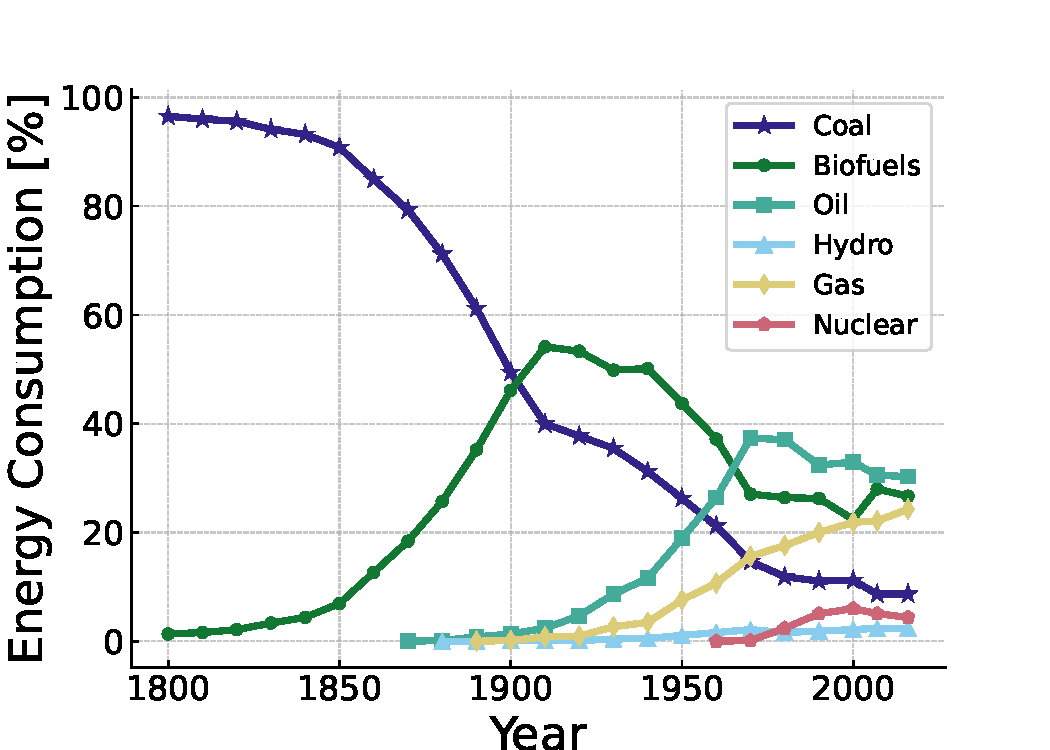
\includegraphics[width=0.499\textwidth]{images/leg_frame/proportional_fuel_use.pdf}
%  }
%   \hfill
%   \subfloat[Total Energy Use.\label{fig:total}]{%
%     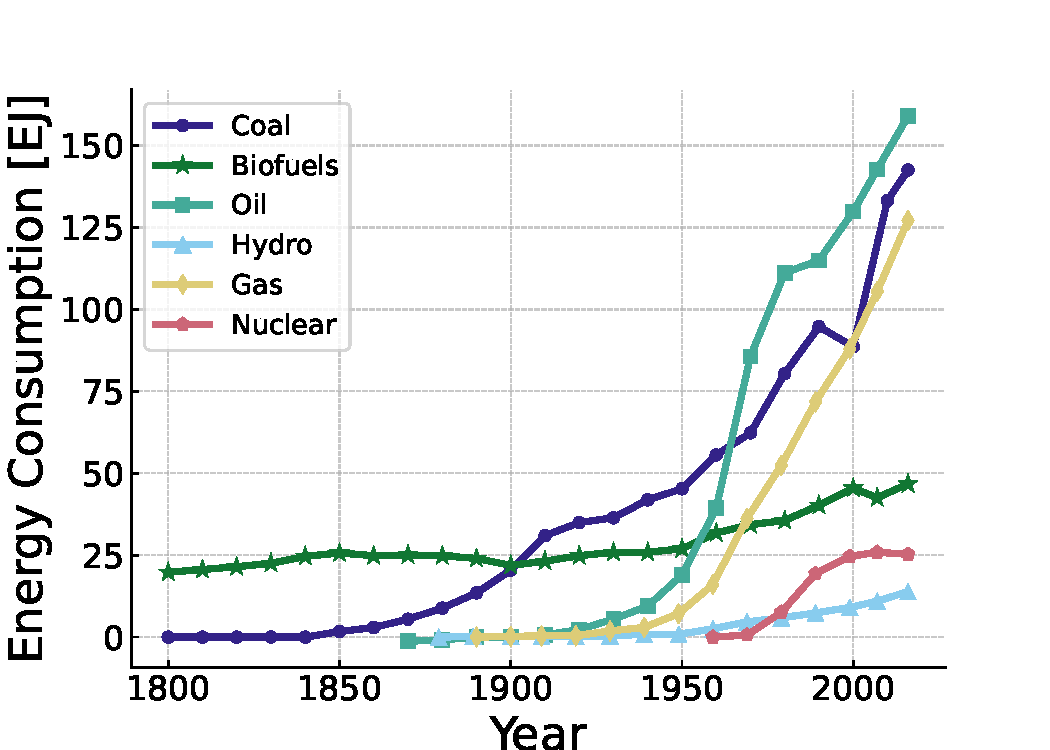
\includegraphics[width=0.499\textwidth]{images/leg_frame/total_fuel_use.pdf}
%  }
%   \caption{
%     Global energy consumption (exajoules) by source from 1800--2017. Reproduced
%     from \cite{york_energy_2019}.}
%   \label{fig:percent_total_energy}
% \end{figure}

% Similarly, what looks in Figure \ref{fig:percent} like a transition away from coal in the early 1900s, with the introduction of alternatives like oil and hydroelectricity, belies the continued increase in coal consumption into the early 2000s. If what we have axiomatically understood as a transition is not happening, we arrive at the kernel of several grand challenges to society and elected officials. The semantic difference between a transition and a displacement is not the core concern; instead, we must focus on realistically presenting the increasing energy needs of society.

% The policy inertia behind the monetary valuation of energy system is something that future generations could overcome, upending the incentives policymakers might implement to drive an actual transition instead of a displacement, as we have discussed. If decision-makers focus on what a policy will do only for the term of their service, they drastically undervalue the impact that daily climate actions will have hundreds of years down the line. We see this dichotomy in the 2020 grid failings in Texas during the unseasonably cold front they experienced. From the outside, we can see how an extreme weather event would create a great demand. This case is a microcosm of a drastic change in a society's values for an energy grid. In a couple of weeks, a state that had praised its sustained grid \cite{texas_ercot_nodate} experienced massive failures only for its service to resume.

% Since 2020, the \gls{ercot} has been working to update its grid to be more resilient to such events. The Grid Deployment Office of the \gls{doe} published a report in 2024 outlining \$270 billion in savings that resulted from increasing connections to the Texas Interconnection \cite{doe_transmission_planning_study_2024}. Concurrent with this announcement, the \gls{doe} announced a \$1.5 billion transmission investment that would go to four projects in Texas, New Mexico, Louisiana, Mississippi, Maine, Oklahoma, and Arizona \cite{doe_tran_announce_2024}. These projects are expected to be completed by 2026 and will increase the grid capacity by 1.5 GW. This is a step in the right direction, but it is not enough to ensure that the grid will be resilient to future extreme weather events.

% We can legislate for such changes by developing policy frameworks that bring in the community and address changing values for energy systems. Elisa Papadis and George Tsatsaronis set out to update the vision for a well-designed policy package in their 2020 paper, surmising that "carefully introduced targeted investment subsidies, performance standards and mandates, communication and education campaigns and a CO$_2$ tax for global aviation and shipping" constitutes achieving this legislative framework \cite{papadis_challenges_2020}. This approach will require geographically bespoke solutions that draw in stakeholders to focus on serving the needs of the future. They advocate for expansion and maintenance investments in the complex \gls{usa} power grid to accommodate flexibly generated capacity.

% Flexibility is a ubiquitous goal of decarbonizing industries, like chemical producers, which highlight big emitters that are large volume/ low-profit goods (disincentivizing development) \cite{mallapragada_decarbonization_2023}, or farm researchers who highlight the growing importance of human intervention as climate change impacts their crop in a negative feedback cycle \cite{farokhi_soofi_farm_2022}. Focusing efforts where investment can have the largest impact in the shortest time and consulting the changing valuation of stakeholders in how modifications to the grid are carried out would further this goal of flexibility.